\documentclass[fleqn,10pt]{wlscirep}
\usepackage[utf8]{inputenc}
\usepackage[T1]{fontenc}
\usepackage{bm}
\usepackage{siunitx}
\DeclareSIUnit{\Bit}{~Bit}
\title{Methode zur Erhöhung der Testkapazität von RT-PCR bei niedrig durchseuchten Proben mittels Samplekombination}

\author[1,*]{Leo T. Peters}
\author[2]{Leonhard Kuboschek}
\author[1,2]{Ruth}
\author[2]{Pranav Kumar Shadamarshan}
\affil[1]{Affiliation, Department, City, Country}
\affil[2]{Affiliation, Department, City, Country}

\affil[*]{e-mail: leo.peters@tum.de}


\begin{abstract}
Diese Arbeit zeigt ein neuartiges Verfahren zur effizienteren Nutzung von PCR-Tests unter der Annahme einer niedrigen Durchseuchung. Dazu werden informationstheroretische Grundlagen auf die Tests medizinischer Größen wie z.B. den Infektionszustand von Patienten angewendet. 
Dazu werden Proben von einzelnen Personen geteilt oder alternativ mehrfach entnommen und mit den Proben anderer Personen gezielt vermischt, um die Testausnutzung (oder informationstheoretisch: die Entropie) der einzelnen Tests zu erhöhen und dadurch die zu untersuchende Gruppe mit dem Einsatz einer geringen Anzahl von Tests vollständig untersuchen zu können. Durch eine rekursive Aufteilung der Testgruppe lassen sich auch alle weitere Tests nahezu optimal nutzen und schließlich einzelne Infizierte ermitteln.
Die im Rahmen dieser Überlegungen durchgeführten Simulationen und analytischen Herleitungen zeigen auf, dass eine lückenlose Testung einer niedrig durchseuchten Gruppe mit weniger Tests als die Anzahl der Gruppenzugehörigen möglich ist. Die Simulationen zeigen auf, dass das Verhältnis aus Anzahl der Patienten einer Gruppe und der Anzahl zur Vermessung der Gruppe einzusetzenden Tests im Mittel abhängig von dem Grad der Durchseuchung ist. Außerdem zeigt sich, dass durch das Verfahren die Spezifität erhöht wird, während die Sensitivität durch die Verdünnung von Proben und die mehrfache Anwendung der PCR geringfügig sinken kann.
\end{abstract}
\begin{document}

\flushbottom
\maketitle

\thispagestyle{empty}

\section*{Introduction}
Die pandemische Verbreitung des Coronavirus SARS-CoV-2 führt weltweit für einen Engpass in der medizinischen Versorgung \cite{Knappheit_med_versorgung}. Darüber hinaus ist die Verfügbarkeit von Tests auf das Virus ein essentieller Bestandteil der Bekämpfung und Verzögerung der Pandemie \cite{TestsBekämpfenCorona}. Gerade im frühen Stadium der Ausbreitung fallen Tests häufig negativ aus, während die Verfügbarkeit der Tests gering ist. Unter diesen Voraussetzungen ist der Informationsgehalt eines einzelnen Tests gering.

Ein einfaches Zahlenbeispiel kann nun verdeutlichen, was dies für die Praxis bedeuten kann: Wenn der Durchseuchungsgrad der Proben an einem bestimmten Tag als $p_inf = \SI{1}{\percent}$ angenommen wird, so erwarten wir in einer durchschnittlichen Charge von 100 Proben eine positive Probe. Um diese mit der Einzeltestung zu vermessen, benötigen wir 100 Tests. Alternativ kann man sich jedoch eine andere Messstrategie vorstellen: Dazu halbieren wir die Probe von jedem Patienten und vermischen eine Hälfte paarweise mit der Probe einer anderen Person und erhalten dadurch 50 Proben-mixe. Die testen wir mit 50 Tests. Wir erhalten im Mittel ein positives Ergebnis und 49 negative Ergebnisse. Dadurch wissen wir, dass 98 Personen negativ sind und können sie nach Hause schicken. Bei den beiden Personen, deren vermischte Probe positiv getestet wurde, werden jetzt einzelne Tests durchgeführt (dafür hatten wir die Proben anfangs halbiert). Mit zwei weiteren Tests wissen, wir wer von beiden oder ob beide positiv sind. Wir haben also im Mittel 52 Tests gebraucht, um 100 Menschen zu testen. Das ganze lässt sich noch weit verbessern und unter informationstheoretischen Annahmen optimieren. Der Versuch einer solchen Optimierung befindet sich im Hauptteil. 

Darüber hinaus stellt sich die Frage, inwiefern durch die neue Teststrategie bzw. -methodik die Verlässlichkeit des Tests verändert wird.

Durch eine Monte-Carlo-Simulation sollen die Fragen nach den mittleren und maximalen Anzahlen von Tests, sowie nach der Verlässlichkeit von Tests abgeschätzt werden.
Dazu werden verschiedene Messstrategien entworfen, optimiert und simuliert.


\section*{Methodik}

\subsection{Optimaler Informationsgehalt und Ansatz für den ersten Test}
Der Informationsgehalt eines Tests entspricht der informationstheoretischen Größe \glqq Entropie\grqq{} $H$ \cite{Shannon} und berechnet sich im Fall des Tests mit binärem Ergebnis aus der relativen Häufigkeit der Infizierten (Durchseuchungsgrad) $p_{inf}$:

\begin{equation}
H(p_{inf}) = -p_{inf} \cdot \log_2(p_{inf})-(1-p_{inf}) \cdot \log_2(p_{inf}) \si{\Bit}
\end{equation}

\begin{figure}[ht]
	\centering
	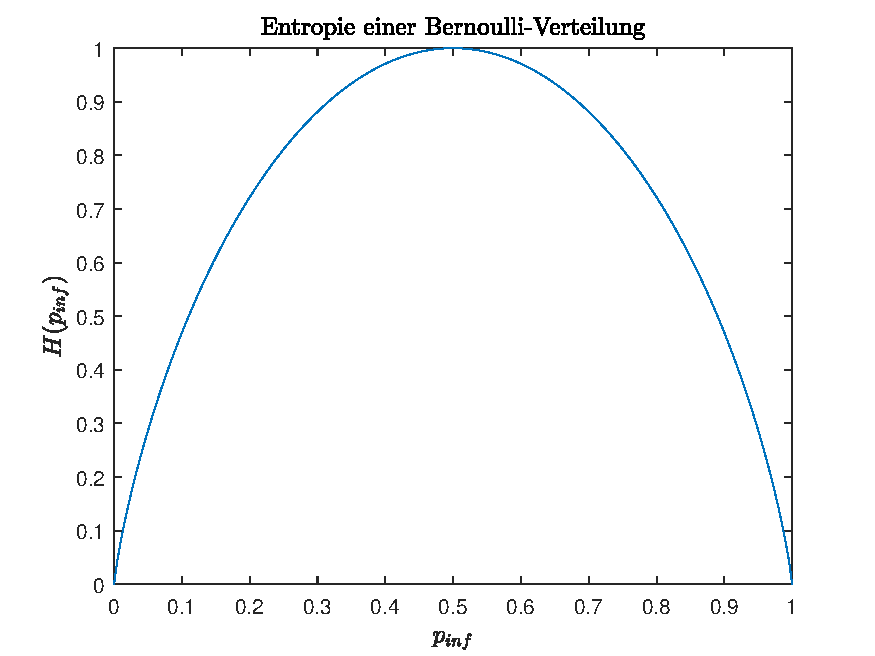
\includegraphics[]{pics/Bin_Entropie.pdf}
	\caption{Informationsgehalt eines Tests mit binärem Ergebnis in Abhängig von dem Durchseuchungsgrad}
	\label{fig:bin_entropie}
\end{figure}

Abb. \ref{fig:bin_entropie} zeigt ein Maximum des Informationsgehaltes eines Tests, wenn die relative Häufigkeit der positiven Testergebnisse $0,5$ beträgt bzw. eine Gleichverteilung vorliegt. Durchseuchungsgrade der Proben oberhalb von $0,5$ werden in dieser Arbeit nicht näher betrachtet, da sich diese auch nicht durch Kombination mit anderen Proben näher zu einer Gleichverteilung erweitern lassen. 

Bei Durchseuchungsgraden kleiner $0,5$ bzw. \SI{50}{\percent} nimmt die Entropie zunächst langsam ab, konvergiert jedoch gerade am Ende schnell gegen Null. Das zeigt, dass ein Test bei einer Einzeltestung der Proben bei niedrigem Durchseuchungsgrad nicht effizient genutzt werden kann.
Durch eine Vermischung von Proben, erhalten wir eine neue Probe, deren Anzahl an positiver Teilproben binomialverteilt ist. Im folgenden wird ein solcher Probenmix als positiv bezeichnet, wenn sich darin mindestens eine positive Teilprobe befindet und sonst negativ. Jede Teilprobe ist stochastisch unabhängig mit der Wahrscheinlichkeit $p_{inf}$ positiv. Die Wahrscheinlichkeit für einen positiven Probenmix lautet nun
\begin{equation}
p_{n,inf}(p_{inf}) = 1-(1-p_{inf})^n 
\end{equation}
wobei $n$ die Anzahl der Teilproben im Probenmix entspricht. Ersichtlich ist, dass durch die Vermischung von Proben der Informationsgehalt eines Tests über den gesamten Mix erhöht werden kann. 

Anhand dieser Gegebenheit lässt sich für einen empirisch ermittelten Durchseuchungsgrad eine Optimale Gruppengröße bestimmen, deren   

\section*{Main text heading 1}

Please use headings/subheadings to break up the text. Main headings should be no more than 38 characters, including spaces.

\subsection*{Subheading 1}

Subheadings should be no more than 39 characters, including spaces. In the final layout, subheadings will be in-line and thus followed by a full stop.

\subsubsection*{Second-level subheading 1}
Second-level subheadings should be no more than 70 characters, including spaces.

\section*{Main text heading 2}

\subsection*{Subheading 2}
\subsubsection*{Second-level subheading 2}
...\\
...

\section*{Outlook/Future Perspectives}
The text is often best rounded off with a comment on the implications of the latest work and on future research directions.  This section should be about 800 words long and is an opportunity for authors to give their vision of where the field is heading.

\section*{7 display items [figures, text boxes or tables]}

Display items should be complementary to the main text and avoid repeating information. Please keep in mind that all display items will need to fit in portrait format. Please cite all display items in the main text. Do any items require copyright permission? If any of the figures have been reproduced or adapted from elsewhere we need you to complete a \href{http://www.nature.com/licenceforms/npg/thirdpartyrights-table.doc}{Third Party Rights Table}, which includes the relevant details (including full reference and figure number) so we can request permission from the publishers to use it.  We do not require the Third Party Rights table to be completed before submission of the first draft.  However, to speed up the process at the author revision step, we recommend that you add the reference numbers to the figure captions.  Please note that we cannot use permissions (to adapt/reproduce figures) that authors have received from publishers. Also, a permission is still required if the author of this Review article is an author of the original manuscript.\\

\noindent For chemical structures, please see the \href {https://www.nature.com/documents/nr-chemical-structures-guide.pdf}{Nature guide for ChemDraw structures}.\\

\noindent For information about the artwork process at Nature Reviews journals, please refer to \href{https://www.nature.com/reviews/pdf/artworkguide.pdf}{the guide to authors} for figures and an  \href{http://www.nature.com/reviews/pdf/artworkguidep2.pdf}{example figure}.\\

\noindent \textbf{Box 1 | Title.}
Word count up to 600 words. Boxes can include small illustrations. Any figures included in boxes should be described in full in the box text — a separate figure caption is not used. Boxes can also contain small tables. Boxes should be included in the manuscript Word document.  Please include them at the end of the article (i.e. the present location in this template) rather than at the position you’d like the box to be in within the main text.  However, please add a call out in the main text for ‘Box 1’.\\

\noindent \textbf{Figure captions}\\
\noindent Please include detailed figure captions that define all symbols and abbreviations used in the figures (e.g. $V$, voltage; $R$, resistance). Readers should understand figures without needing to refer to the text. Figure captions should be included in the manuscript latex document. Figures should be provided separately.\\

\begin{figure}[ht]
\centering
%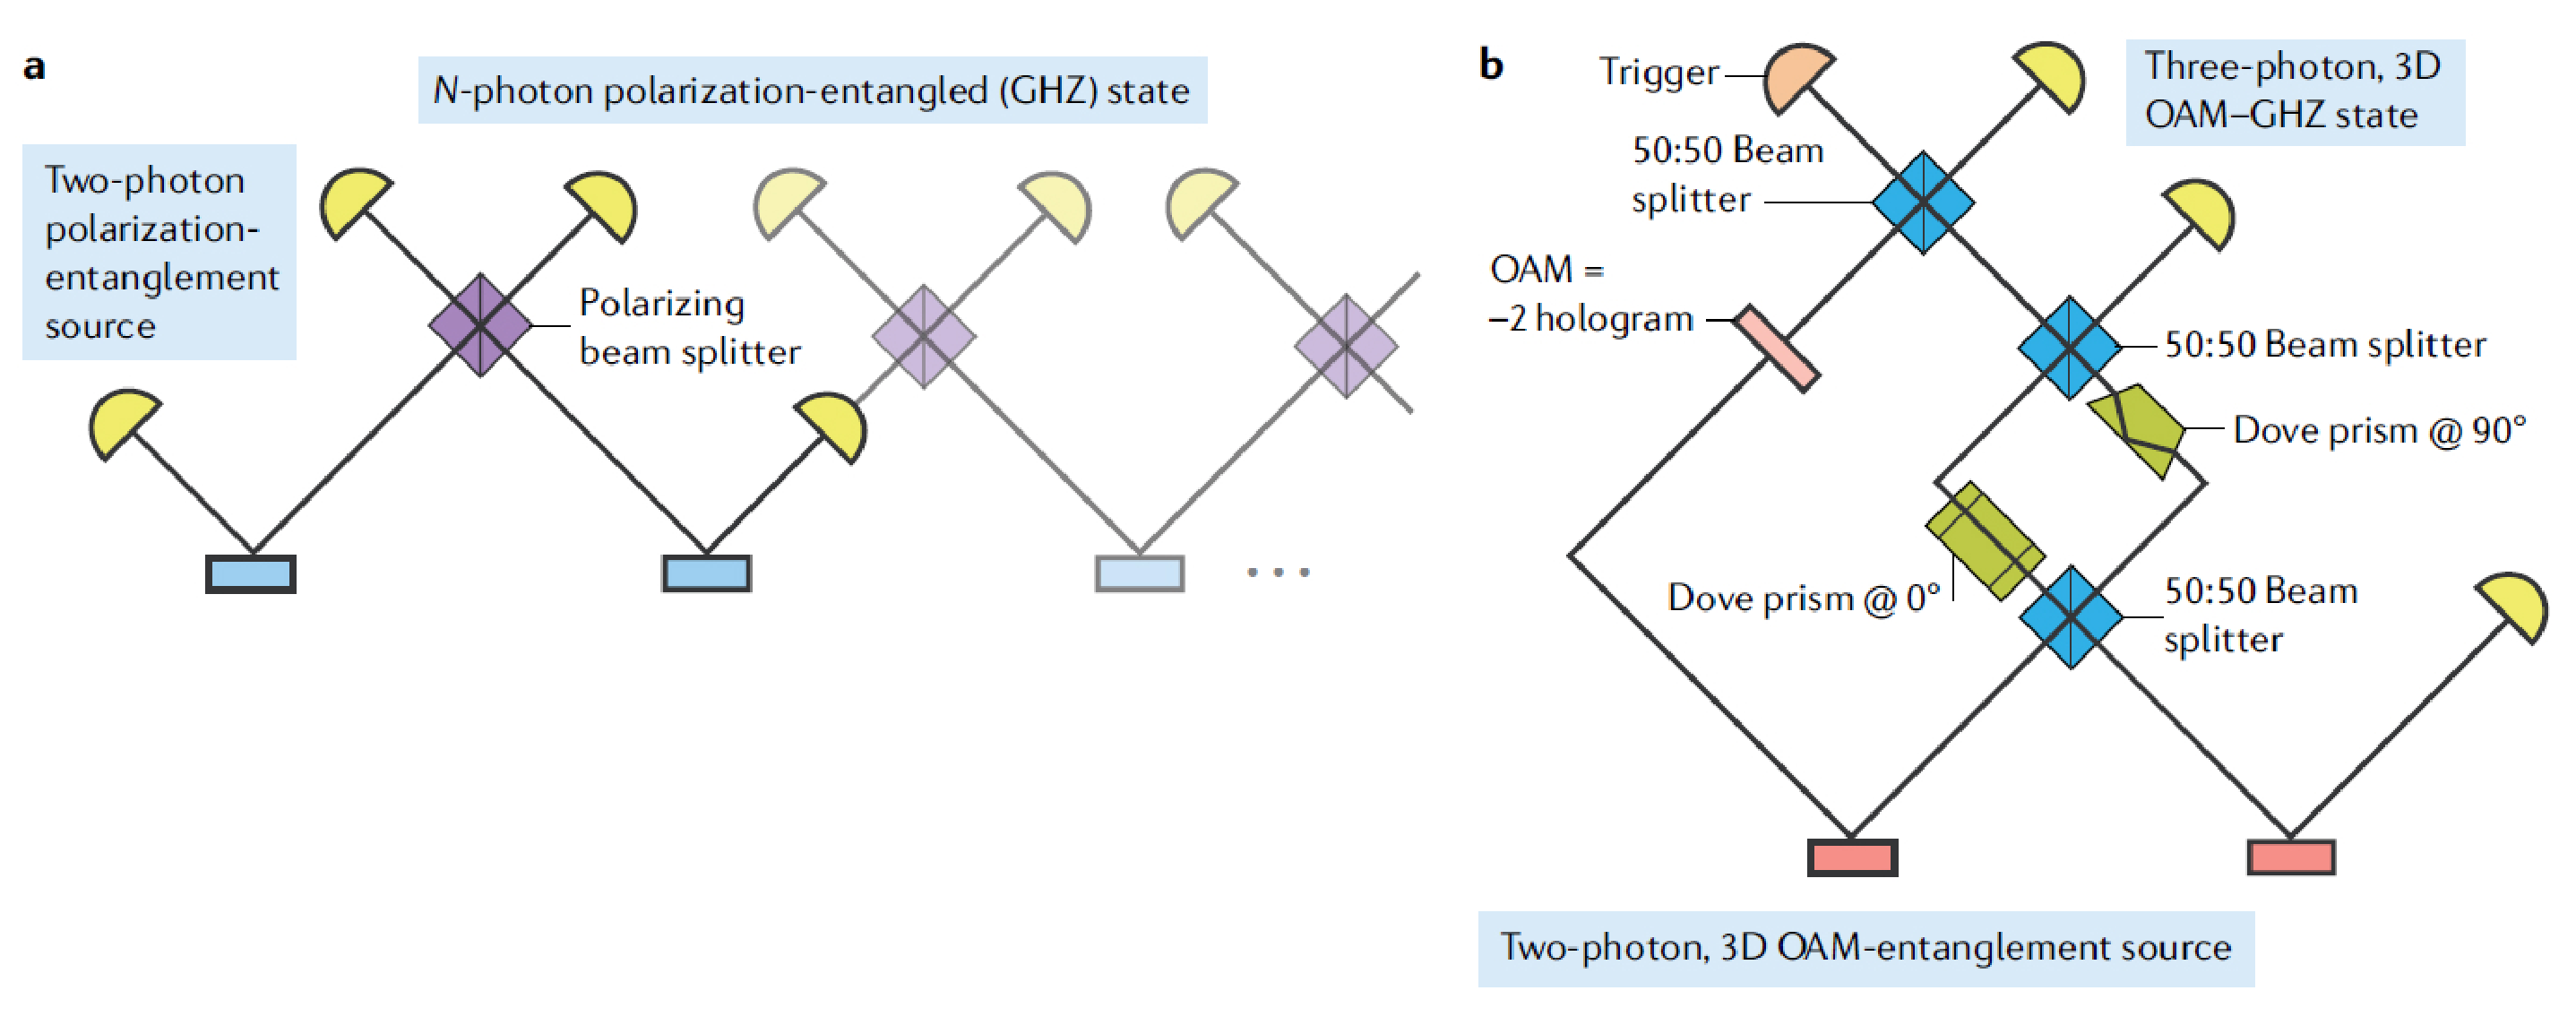
\includegraphics[width=\linewidth]{fig}
\caption{\textbf{Title.} a | Text. b | Text. c | Text. d | Text maximum 250 words. Panel a is adapted/reproduced with permission from ref.123, Springer Nature Limited. Panel b is adapted/reproduced with permission from ref.124, Publisher Name.}
\label{fig}
\end{figure}



\begin{table}[ht]
\centering
\begin{tabular}{|l|l|l|}
\hline
Particle & Mass & Charge \\
\hline
 \multicolumn{3}{|c|}{Charged particles}\\
\hline
Electron & $9.10938356(11)\times10^{-31}$ kg & $-1e$ \\
\hline
Proton & $1.672621898(21)\times10^{-27}$ kg & $+1e$ \\
\hline
 \multicolumn{3}{|c|}{Neutral particles}\\
\hline
Neutron & $1.674927471(21)\times10^{-27}$ kg & $0$ \\
\hline
\end{tabular}
\caption{\label{tab}Tables have titles but no captions are allowed. All symbols and acronyms used in a table should be defined in a footnote. Example: Here $e$ is the elementary charge.}
\end{table}


\section*{References} 

150–200 references are suggested. All referenced work should be accepted for publication or on recognized Archive databases. References should be given superscript numbers and cited sequentially according to where they appear in the main text, followed by those in the text boxes, figure captions and then tables (i.e. the order they appear in this template).
Journal abbreviation in italics, volume number in bold. If there are six or more authors for a reference, only the first author should be listed, followed by 'et al.'. Journal name abbreviations are followed by a full stop. Please include full page ranges. \\

\noindent Please do not cite web sites in the reference list — these should be listed separately, with the URLs in the Related Links section (see below).  If you are unsure if the website is a ‘Related link’ or should go in the ‘References’ section then identify if there is a publication date on the website.  If there is a publication date, it is likely that the item will be in the ‘References’ section.  If there is no publication date, it is likely that the item will be in the ‘Related Links’ section.\\

\noindent When citing a book, please indicate if you are citing a specific page range or chapter.  Otherwise, we presume that you are citing the entire book.  \\

\noindent \textbf{Highlighted references (optional)} Please select 5–-10 key references and provide a single sentence for each, highlighting the significance of the work.\\

\noindent\textbf{Acknowledgements}\\
E.g. Funding agencies.\\

\noindent\textbf{Author contributions}\\
Please describe the contributions made by each author.  Please use the initials of the individual author to explain these contributions.  These contributions are also required when you upload the files to our submission website.\\

\noindent\textbf{Competing interests}\\
Nature Journals require authors to declare any competing interests in relation to the work described. Information on this policy is available \href{http://www.nature.com/authors/policies/competing.html}{here}. \\



\noindent\textbf{Supplementary information (optional)}
If your article requires supplementary information, please include these files for peer-review. Please note that supplementary information will not be edited.


\end{document}